%!TEX root = thesis.tex


\chapter{Data}
\label{chap:data}

\section{Vector data}
\subsection{Topography}
\begin{sloppypar}
	The datasets of Dutch provinces (provincies, Figure \ref{fig:provinces}) and municipalities (gemeenten, Figure \ref{fig:municipalities}) have been downloaded from \url{https://www.pdok.nl/nl/producten/pdok-downloads/basis-registratie-kadaster/bestuurlijke-grenzen-actueel}. For the Netherlands there are 12 features in the provinces and 393 in the municipalities dataset. 
	
	It has been challenging to obtain data of administrative boundaries of Belgium (even from the \ac{inspire} data portal). Therefore, all data for Belgium was retrieved from \url{http://www.gadm.org/}. There are also 12 features in the provinces (including the capitol region of Brussels) and there are 589 features in the municipalities dataset.  
	
	The country datasets have also been downloaded from \url{http://www.gadm.org/} (Figure \ref{fig:countries}). The administrative unit data contains the names of the administrative units and their (polygon) geometry. 
\end{sloppypar}

\subsection{Land cover}
\begin{sloppypar}
	Data on land cover will be used to complement the data of administrative units. A section of the 2012 dataset from the \ac{corine} programme will has been selected for this (Figure \ref{fig:CORINE}). The entire CORINE dataset was retrieved from \url{http://land.copernicus.eu/pan-european/corine-land-cover/clc-2012}. The features overlapping the Netherlands and Belgium have been retrieved from this dataset using the open source QGIS software and stored in a separate database in Postgres. 
	
	The database contains polygon geometries (Figure \ref{fig:CORINEZOOM}) with a unique identifier and a code that refers to the type of landcover. These codes can be looked up in the accompanied spreadsheet file containing the legend table of \ac{corine} 2012.  	
\end{sloppypar}

\section{Raster data}
Data is often used in a raster representation for computations in a \ac{gis}. For natural phenomenon a raster representation is especially well suited. The \ac{eea} reference grid is a standard grid which covers Europe. It is available with a resolution of 100km\textsuperscript{2}, 10km\textsuperscript{2} and 1km\textsuperscript{2}. In this thesis the \ac{eea} grid cells with a resolution of 100km\textsuperscript{2} (Figure \ref{fig:100KM}) and 10km\textsuperscript{2} (Figure \ref{fig:10KM}) have been used that overlap the Netherlands and Belgium. 15 grid cells of 100km\textsuperscript{2} and 843 grid cells of 10km\textsuperscript{2} have been selected from the original dataset.  

\begin{figure}
	\centering
	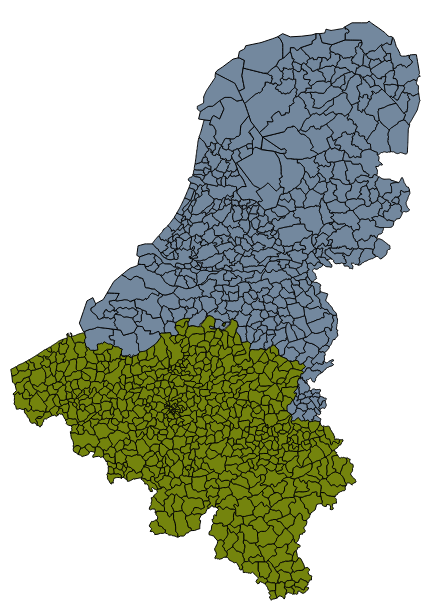
\includegraphics[width=0.5\linewidth]{figs/Municipalities.png}
	\caption{Dataset of municipalities in the Netherlands and Belgium in 2015 (from Dutch cadaster and GADM.org)}
	\label{fig:municipalities}
\end{figure}

\begin{figure}
	\centering
	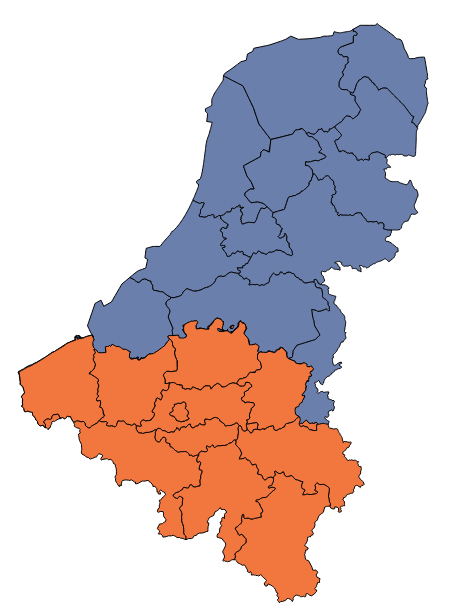
\includegraphics[width=0.5\linewidth]{figs/Provinces.png}
	\caption{Dataset of provinces in the Netherlands and Belgium in 2015 (from Dutch cadaster and GADM.org)}
	\label{fig:provinces}
\end{figure}

\begin{figure}
	\centering
	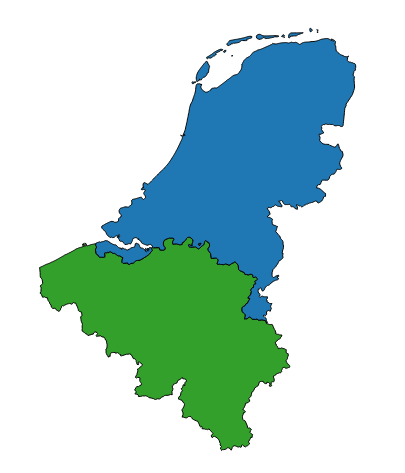
\includegraphics[width=0.5\linewidth]{figs/Countries.png}
	\caption{Dataset of the Netherlands and Belgium in 2015 (from GADM.org)}
	\label{fig:countries}
\end{figure}

\begin{figure}
	\centering
	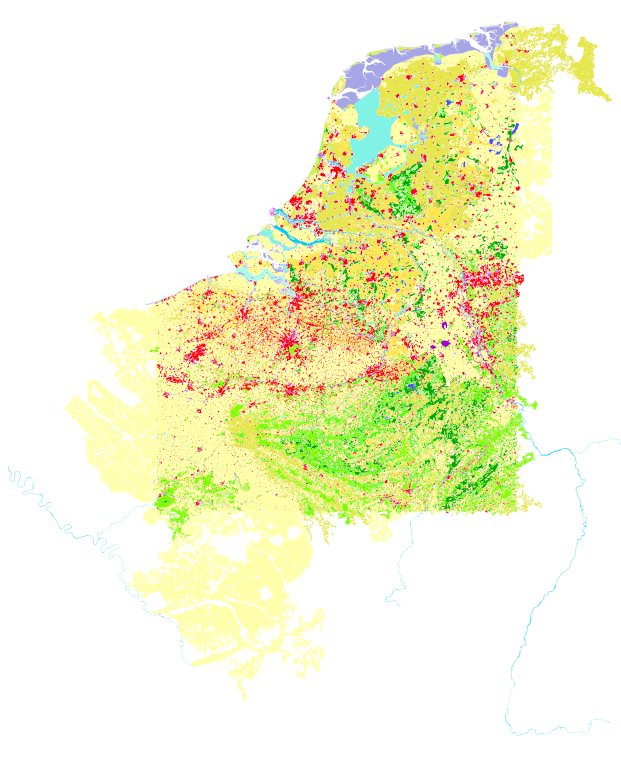
\includegraphics[width=1\linewidth]{figs/CORINE_NL_BE_color.PNG}
	\caption{Dataset of landcover in the Netherlands and Belgium in 2012 (from Copernicus  The European Earth Observation Programme)}
	\label{fig:CORINE}
\end{figure}

\begin{figure}
	\centering
	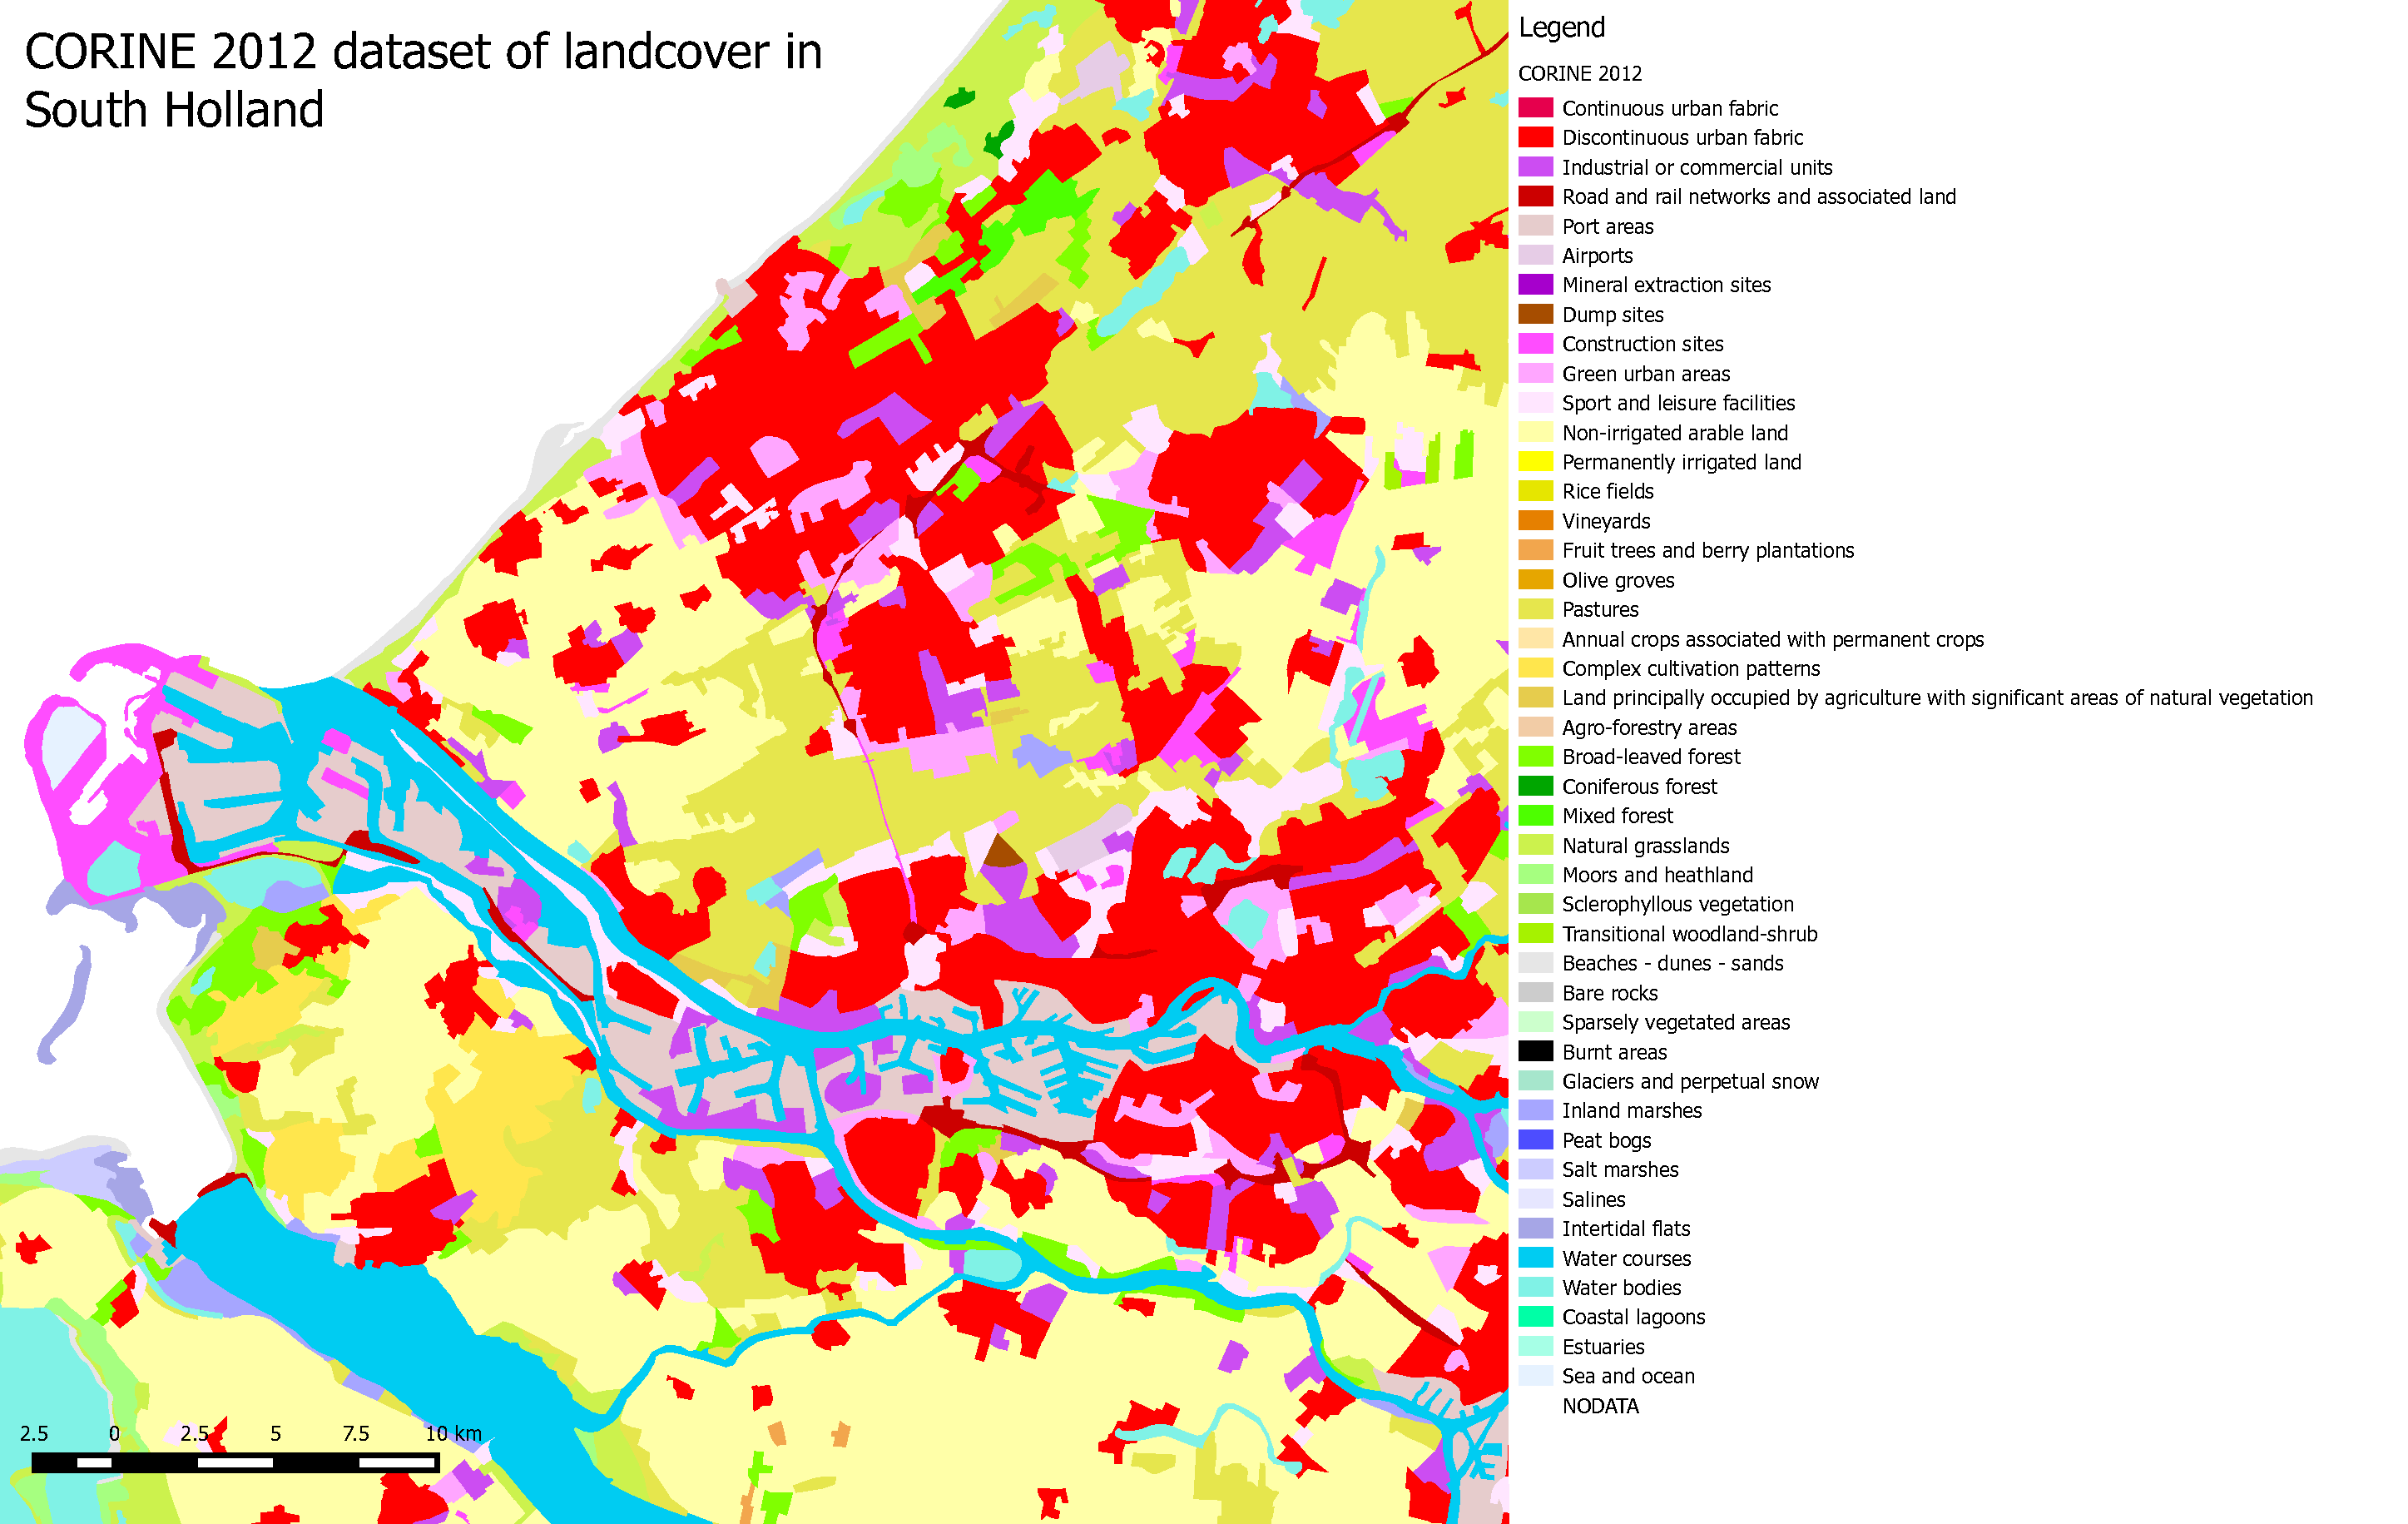
\includegraphics[width=1\linewidth]{figs/CORINE_NL_BE_color_zoom.PDF}
	\caption{Landcover of the province of South Holland (subsection of the dataset from Figure \ref{fig:CORINE})}
	\label{fig:CORINEZOOM}
\end{figure}

\begin{figure}
	\centering
	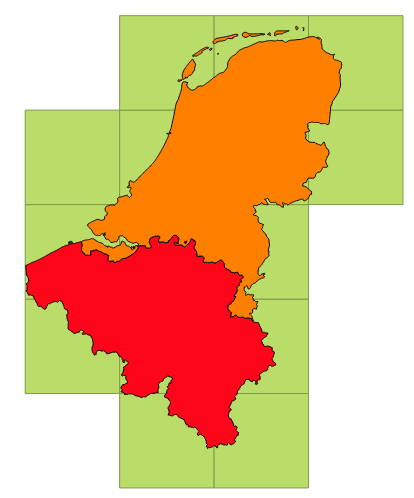
\includegraphics[width=0.7\linewidth]{figs/EEA100km.png}
	\caption{\ac{eea} reference grid cells with a resolution of 100km\textsuperscript{2} overlapping the Netherlands and Belgium}
	\label{fig:100KM}
\end{figure}

\begin{figure}
	\centering
	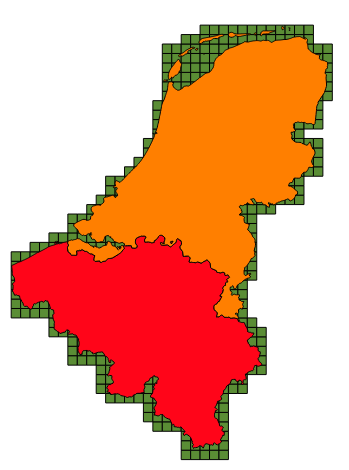
\includegraphics[width=0.7\linewidth]{figs/EEA10km.png}
	\caption{\ac{eea} reference grid cells with a resolution of 10km\textsuperscript{2} overlapping the Netherlands and Belgium}
	\label{fig:10KM}
\end{figure}

\section{Sensor data}
Air quality sensor data will be used from the \ac{rivm} (\url{http://inspire.rivm.nl/sos/}) and from the \ac{ircel} (\url{http://sos.irceline.be/}). Both of these organisations have a \ac{sos} where data can be retrieved according to the \ac{swe} standards. The one of the \ac{rivm} has been online since the 21\textsuperscript{st} of August, 2015. \ac{ircel} already made the \ac{sos} available on the first of January, 2011. Figure \ref{fig:RIVMSensor} and Figure \ref{fig:IRCELINESensor} show the sensor networks of both organisations. They provide different kinds of sensor data, such as particulate matter ($PM_{10}$), nitrogen dioxide ($NO^{2}$) and ozone ($O^{3}$). Figure \ref{fig:Sensor} shows one of the sensor locations in the city center of Amsterdam. 


\begin{figure}
	\centering
	\includegraphics[width=0.6\linewidth]{figs/RIVMSensors.png}
	\caption{Webmap by the \ac{rivm} showing their air quality sensor network (\url{http://www.lml.rivm.nl/meetnet})}
	\label{fig:RIVMSensor}
\end{figure}

\begin{figure}
	\centering
	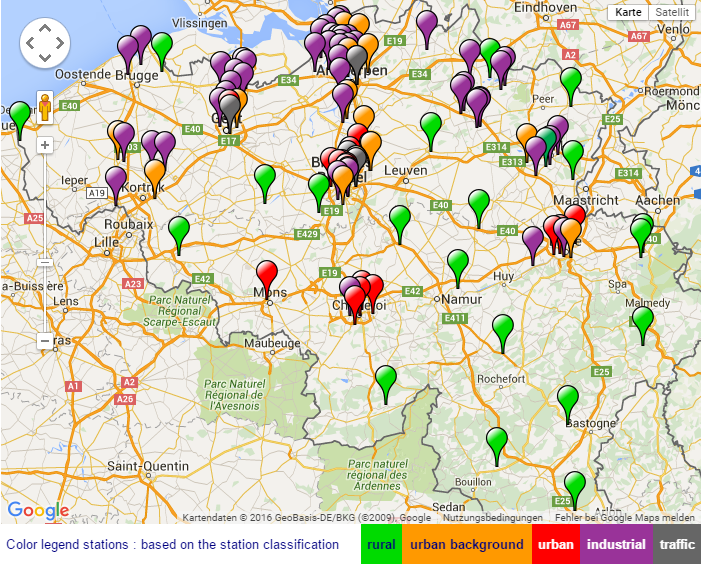
\includegraphics[width=0.6\linewidth]{figs/IRCELINESensors.png}
	\caption{Webmap by \ac{ircel} showing their air quality sensor network (\url{http://www.irceline.be/en/air-quality/measurements/monitoring-stations/})}
	\label{fig:IRCELINESensor}
\end{figure}

\begin{figure}
	\centering
	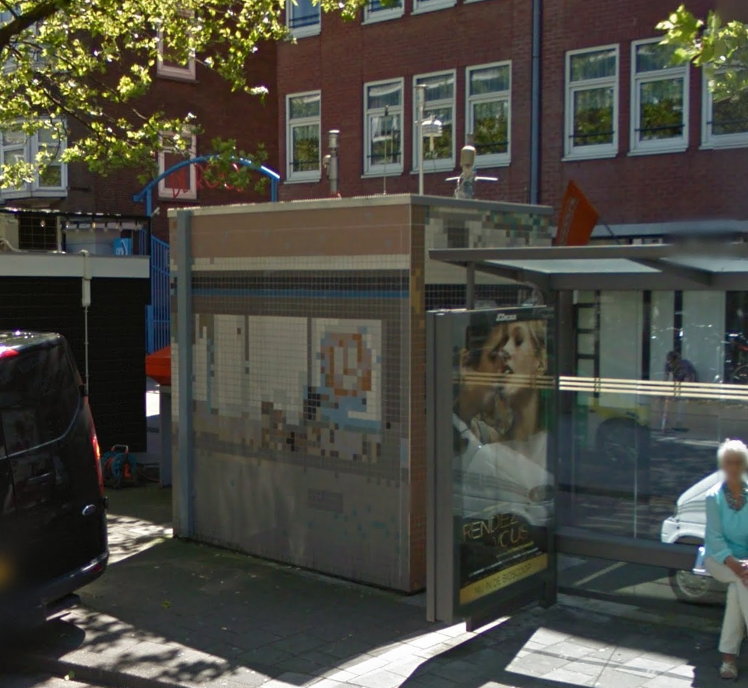
\includegraphics[width=1\linewidth]{figs/SensorAdam.png}
	\caption{Google Streetview image of \ac{rivm} sensor location in Amsterdam in 2015}
	\label{fig:Sensor}
\end{figure}
